\documentclass{article}
\usepackage{ragged2e}
\usepackage{graphicx}
\graphicspath{ {C:\Users\goyf\Desktop\projects\OpAmp} }
\usepackage[utf8]{inputenc}
\usepackage[english]{babel}
\usepackage{float}
\usepackage{hyperref}

\usepackage{cite}



%\author{Jan Polivka}
\date{\vspace{-5ex}}

\begin{document}
 	\title{LEDs and comparators}

	\maketitle
	\section{What this project is about}
	Many of us have issues studying OpAmps as they seem almost intangible
	as they are usually more hidden within electrical structures without
	an apparent use from the point of view of the student.
	This project is about constructing a simple OpAmp circuit to make the
	device a little more approachable.

	\section{Components and circuit scheme}
		\subsection{Components}
		\begin{itemize}
		\item 2 LM741 OpAmps
		\item 2 150 Ohm Resistors 
		\item 2 Potentiometers	
		\item 2 LEDs
		\end{itemize}

		\subsection{Circuit Scheme}
		\begin{figure}[H]
			\centering
			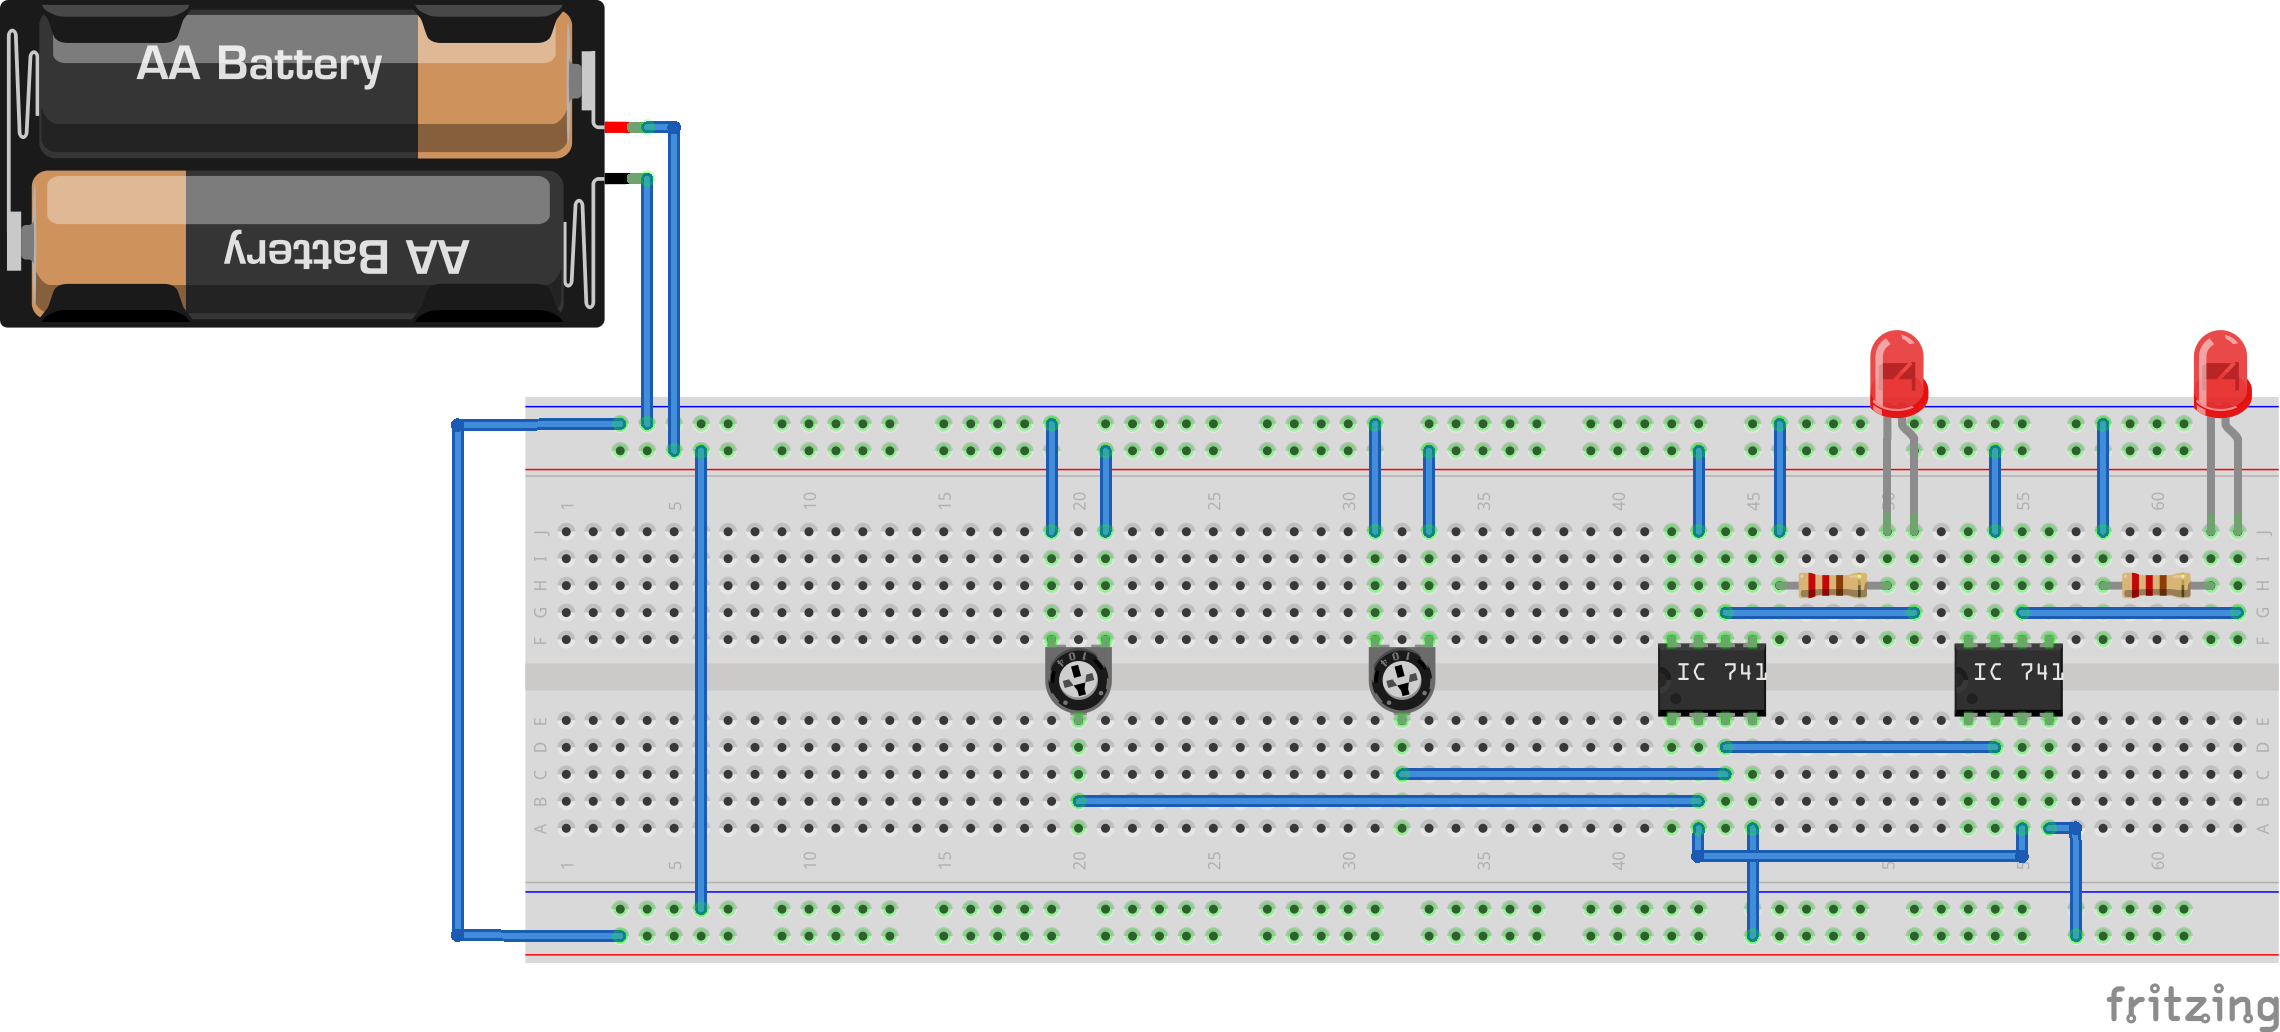
\includegraphics[scale=0.45]{circuit_bb}
			\caption{OpAmp comparator circuit \cite{circuit}}
		\end{figure}

	\section{How it works}
	The circuit is based on two differential OpAmps which serve as comparators.
	An OpAmp compares the voltages on the 10K resistor	and outputs the difference 
	multiplied by the gain of the OpAmp. If the	voltage output is positive, it will cause
 	the LED to light up and because one of the OpAmps is inverting and the other is not,
	they will each produce voltage of opposite signs, causing one LED to light up while the other is not.

	\section{Why it works}
	\subsection{Differential OpAmp}

	To explain in greater how an OpAmp works, the function of a bipolar junction transitior
	must be cleared up first.

	\begin{figure}[H]
		\centering
		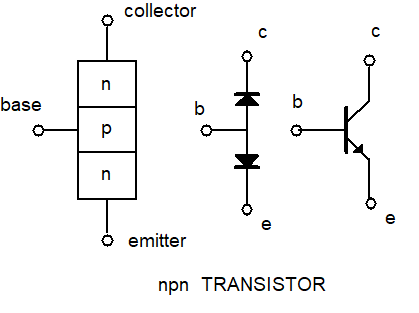
\includegraphics{bjt}
		\caption{Bipolar Junction Transistor}
	\end{figure}

	A BJT is composed of two pn-diodes back-to-back, creating an npn bridge.
	The device itself work when a small current is injected in to the base
	which causes a large current to flow from the collector to the emitter.
	What is happening in terms of electrons is that when a positive terminal
	is connected to the base, electrons will move from the emitter to the base
	and only a very few electrons will combine with the holes, the rest will
	jump to the collector layer due to their kinetic energy.

	\begin{figure}[H]
		\centering
		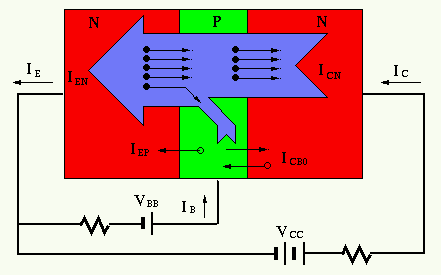
\includegraphics[scale=0.75]{bjtelectrons2}
		\caption{Current and Electrons in a BJT\cite{bjt}}
	\end{figure}

	The current on the collector is given by the relationship

	\[I_C = {\beta}I_B \]

	Beta is a parameter of the particular component as is given in a range, e.g. 40 - 800.

	\[I_E = I_C + I_B \]

	For most cases \[I_E \approx I_C\]

	Now that the function of an OpAmp is known, it is time to move on to the
	OpAmp itself.

	\begin{figure}[H]
		\centering
		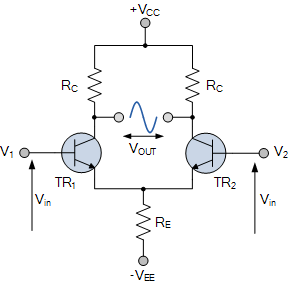
\includegraphics[scale=0.75]{OABones}
		\caption{Differential OpAmp circuit\cite{diff}}
	\end{figure}

	Two important things are going on in here. First, the current coming from Vcc
	has to split into two according to the Current Div Rule. Second, there are
	different currents injected in to the bases of the transistors causing the two
	collector currents to be different.

	\begin{figure}[H]
		\centering
		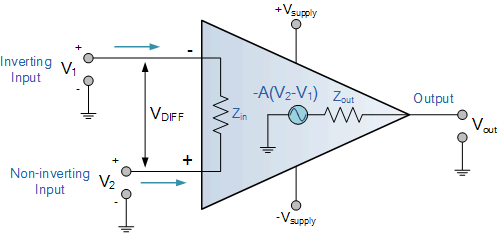
\includegraphics[scale=0.75]{OAAbs}
		\caption{Differential OpAmp abstracted scheme\cite{diff}}
	\end{figure}

	This is a simplified model of an OpAmp. A couple of things to note:

	Z\textsubscript{IN} is infinite, Z\textsubscript{OUT} is zero and the gain is governed by the relation

	\[V_{OUT} = A_V(v_+ - v_-) \]

	A\textsubscript{V} is the gain and is the ratio between V\textsubscript{OUT} and V\textsubscript{IN}.

	\section{Conclusion}
	In this project, a comparator circuit was constructed
	to make OpAmps more approachable and to explain the function of the
	differential amplifier. Feel free to leave any feedback.

	\section{Sources}

	\begin{thebibliography}{3}

	\bibitem{circuit} 
	Dark and Light Indicator Circuit using OpAmp IC LM358,
	\\\texttt{https://circuitdigest.com/electronic-circuits/dark-and-light-indicator}

	\bibitem{bjt} 
	Bipolar Junction Transistor (BJT),
	\\\texttt{http://fourier.eng.hmc.edu/e84/lectures/ch4/node3.html}

	\bibitem{diff} 
	Operational Amplifier Basics,
	\\\texttt{http://www.electronics-tutorials.ws/opamp/opamp\_1.html}

	

	\end{thebibliography}

\end{document}


